%%%%%%%%%%%%%%%%%%%%%%%%%%%%%%%%%%%%%%%%%%%%%%%%%%%%%%%%%%%%%%%%%%%%%%%%%%%

\documentclass{standalone}

\usepackage{amsmath}
\usepackage{mathptmx}
\usepackage{pgfplots}
\usetikzlibrary{external}
\tikzexternalize{a1-bminus4-c10}
\pgfplotsset{compat=1.15}

%% IEEE uses Times Roman font, so we'll default to Times.
%% These three commands make up the entire times.sty package.
\renewcommand{\rmdefault}{ptm}
\renewcommand{\ttdefault}{pcr}
\normalfont\selectfont

\newcommand{\comma}{,\,}
\newcommand{\tuple}[2]{\left({#1}\comma {#2}\right)}

\begin{document}

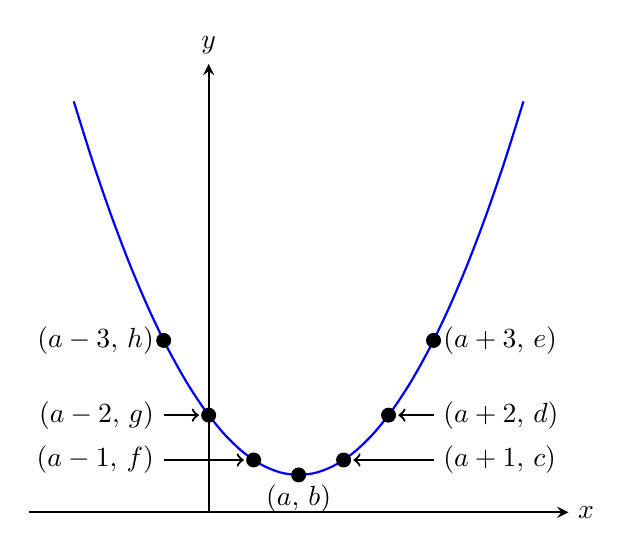
\begin{tikzpicture}
\tikzset{%%
  every mark/.append style={scale=1.0},%%
  scale=1.0%%
}
\pgfplotsset{%%
  every axis/.append style={font=\normalsize}%%
}
%%
\begin{axis}[%%
  axis line style=thick,%%
  axis lines=center,%%
  dotStyle/.style={only marks,mark size=2.5,black,mark color=black,mark=*},%%
  enlargelimits=true,%%
  plotStyle/.style={%%
    domain=-3:7,%%
    mark=none,%%
    smooth,%%
    thick%%
  },%%
  ticks=none,%%
  %%
  %% x-axis
  xlabel={\normalsize $x$},%%
  xlabel style=right,%%
  %%
  %% y-axis
  ylabel={\normalsize $y$},%%
  ylabel style=above%%
]
%%
%%
%% The function f(x) = x^2 - 4x + 10.
\addplot+ [plotStyle]
{x^2 - 4*x + 10};
%%
%% Some points on the graph of f(x).
\addplot[dotStyle] coordinates {
  (-1,15)  %% A
  (0,10)   %% B
  (1,7)    %% C
  (2,6)    %% D
  (3,7)    %% E
  (4,10)   %% F
  (5,15)   %% G
};
%%
%% Label the above points.
\node[left] at (axis cs:-1,15) {$\tuple{a-3}{h}$};
%%
\node[left] (minusTwo) at (axis cs:-1,10) {$\tuple{a-2}{g}$};
\node[] (B) at (0,10) {};
\draw[->,thick] (minusTwo) -- (B);
%%
\node[left] (minusOne) at (axis cs:-1,7) {$\tuple{a-1}{f}$};
\node[] (C) at (1,7) {};
\draw[->,thick] (minusOne) -- (C);
%%
\node[below] at (axis cs:2,6) {$\tuple{a}{b}$};
%%
\node[right] (plusOne) at (axis cs:5,7) {$\tuple{a+1}{c}$};
\node[] (E) at (3,7) {};
\draw[->,thick] (plusOne) -- (E);
%%
\node[right] (plusTwo) at (axis cs:5,10) {$\tuple{a+2}{d}$};
\node[] (F) at (4,10) {};
\draw[->,thick] (plusTwo) -- (F);
%%
\node[right] at (axis cs:5,15) {$\tuple{a+3}{e}$};
\end{axis}
\end{tikzpicture}

\end{document}
